\documentclass[
	%a4paper, % Use A4 paper size
	letterpaper, % Use US letter paper size
]{jdf}
\newcommand{\pcite}[1]{(\cite{#1})}
\addbibresource{../../references.bib}
\author{William Luna}
\email{wluna6@gatech.edu}
\title{Assignment 2: Research Log}

\begin{document}
%\lsstyle

\maketitle

\section{Background}
% In about half a page, summarize your current state. This would largely cover where you left off last week.
Picking up from last week's \textbf{Planning} section, I felt that my literature review validated the desire to leverage an LLM to create graded reading content for second language learners. Those papers provided evidence that there is a need for such a tool, that building one seems technically feasible, and that there are multiple potential principles in learning science to leverage.

This leaves me curious about the potential intersection between Extensive Reading and Spaced Repetition Software. Last week's research brought the following observations:

\begin{enumerate}
    \item It takes about seventeen exposures over several months to dedicate a new vocabulary word to long-term memory.
    \item Most graded readers are usually much shorter than regular books, and can be read in the span of days or weeks of dedicated daily reading time.
    \item Any single graded reader tends to repeat the same vocabulary words.
\end{enumerate}

Are these observations that vocabulary acquisition could be improved by creating graded readers that have continuity in their vocabulary across many books that take months to read, that can present vocabulary at ideal intervals?

There are some additional lingering questions I will explore:

\begin{enumerate}
    \item How well can LLMs analyze the linguistic complexity of a text?
    \item Dictionary use helps and hinders reading. Can we reach a conclusion on whether its conclusion is a net benefit or detractor to learning vocabulary through extensive reading?
    \item What are the technical implementation challenges in building such a system? Are there recommendations in terms of APIs and/or frameworks?
    \item What is the best means of parsing the text generated by an LLM, particularly boundaries between words and idioms?
\end{enumerate}

\section{Papers and Other Reference Material}
%As you walk through the Research Guide, you’ll be finding lots of papers to read. Here, you’ll make a list of the papers you come across and give considerable attention to. We would expect the Research Log to include at least 15-20 sources (though more is fine as well), and at least 12 (preferably more) should be academic and peer-reviewed. You may include blog posts, newspaper articles, etc. as well, but you should have at least 12 academic sources, too.

\subsection{\fullcite{caines2023application}}
%The paper’s bibliographic information (its APA citation, typically)
\subsubsection{Identification}
%In around one sentence, how you found it (a Google Scholar search? From a conference’s proceedings? From another paper’s references? %Something else?)
Prompted Chat GPT to provide papers on dynamic text generation for the purpose of foreign language learning.

\subsubsection{Summary}
%In around three sentences, a brief, original summary in your own words
This paper is a literature and technical review of how Large Language Models are being leveraged for language education. It covers several models, including BERT, BART, and T5, companies such as Duolingo, Minerva, and Google, and use cases, such as automatic grading, evaluating teaching materials, and live tutoring. The paper concludes with a section on risks and ethical considerations, bringing up bias towards English and climate impact, but with the overall sentiment that LLMs stand to have a transformative and positive impact on language learning. 

\subsubsection{Takeaways}
%In around three sentences, the main takeaways going forward
This paper provided minimal insight and the greatest takeaway was that literature reviews that don't conduct an experiment to validate a hypothesis f their own may have limited utility during the rest of this research phase. It does confirm many already-held beliefs about the utility of LLMs in language learning. In the event that Open AI's 4o language model is cost-prohibitive to use for this project, it does provide the names of several other providers to explore.

\subsection{\fullcite{pilán2016readable}}
%The paper’s bibliographic information (its APA citation, typically)
\subsubsection{Identification}
%In around one sentence, how you found it (a Google Scholar search? From a conference’s proceedings? From another paper’s references? %Something else?)
This paper was provided from the same Chat GPT search as the one above.

\subsubsection{Summary}
%In around three sentences, a brief, original summary in your own words
Provides a summary of the evolution of frameworks used to benchmark the linguistic complexity of text, with an emphasis on Swedish. The traditional Swedish readability measure LIX is deemed insufficiently sophisticated and a supervised machine learning model is implemented and tested. This model is evaluated and considered best in class based on several benchmarks for other languages. The paper points out challenges unique to sentence- vs. document-level benchmarking.

\subsubsection{Takeaways}
%In around three sentences, the main takeaways going forward
Paper is too old to make a comment specifically on LLMs' performance at complexity assessment. However, the fact that a machine learning algorithm can outperform a rules-based method bodes well, since last week's research provided multiple examples of an LLM outperforming neural networks and no cases of an ML algorithm maintaining dominance for NLP tasks. There are some follow-up questions around the appropriate gradations of linguistic complexity: the model is trained on the European A1-C2 framework but there was no evidence to suggest these levels are sufficiently granular to represent phases of \textit{learning}, only \textit{fluency}.

\subsection{\fullcite{liu2023lost}}
%The paper’s bibliographic information (its APA citation, typically)
\subsubsection{Identification}
%In around one sentence, how you found it (a Google Scholar search? From a conference’s proceedings? From another paper’s references? %Something else?)
Found this paper searching google for papers focused on examining how many words map onto how many tokens of a context window, and to what extent LLM retrieval degrades as a function of longer context windows.

\subsubsection{Summary}
%In around three sentences, a brief, original summary in your own words
Rough heuristic of four tokens equating to three words is provided, since most words are one token but compound words and punctuation require additional tokens. The more illuminating finding is that LLMs are best at retrieving information found at the beginning or the end of a text input, where concepts explored in the middle sections struggle to be summarized as accurately. Paper concludes that while fine-tuning can alleviate some challenges in mid-input retrieval, shorter context windows and/or chaining together shorter prompts may be necessary to preserve consistent memory of all text shown to an LLM.

\subsubsection{Takeaways}
%In around three sentences, the main takeaways going forward
Given that my proposed system will be focused on teaching language, likely by fabricating a work of fiction, accurate retrieval is unlikely to be important enough for this finding to cause much concern. However, paired with GPT-4 pricing data and the observation that every three words use four tokens, it does create incentive to default to short prompts and inputs when building this system. For example, after the LLM has generated 3,000 words, rather than feed it the entire story it has written so far as context, it may make more sense to only provide an ongoing summary and the most recent few hundred words.

\subsection{\fullcite{mlq2023tokens}}
%The paper’s bibliographic information (its APA citation, typically)
\subsubsection{Identification}
%In around one sentence, how you found it (a Google Scholar search? From a conference’s proceedings? From another paper’s references? %Something else?)
Found from the same Google search. Not a research paper but seemed very informative.

\subsubsection{Summary}
%In around three sentences, a brief, original summary in your own words
This blog post is a fantastic primer on GPT's approach to tokenization, including the distinction between word- and subword-based segmentation. The context windows of all state-of-the-art LLMs are compared with a discussion of the tradeoffs of each. Different use cases are provided to illustrate when each model might be the best candidate for those specific tasks.

\subsubsection{Takeaways}
%In around three sentences, the main takeaways going forward
One take away is that–if price is no object–I don't need to be worried about context windows since it's unlikely for my project to produce a single text of anywhere near one hundred thousand words, the approximate context window of GPT-4 Turbo. A higher-level takeaway is that one cannot assume that all tokenization approaches are created equal, which may mean that some LLM pricing models are considerably more expensive than they let on (if they use sub-word tokenization, for example).

\subsection{\fullcite{cepedasrs}}
%The paper’s bibliographic information (its APA citation, typically)
\subsubsection{Identification}
%In around one sentence, how you found it (a Google Scholar search? From a conference’s proceedings? From another paper’s references? %Something else?)
Found this paper from a Google Scholar search for studies on the efficacy of spaced repetition in cementing vocabulary into long-term memory.

\subsubsection{Summary}
%In around three sentences, a brief, original summary in your own words
The study claims that "if you want to know the optimal distribution of your study time, you need to decide how long you wish to remember something." While it uses the terminology of Gap and Retention Intervals, the more sobering observation was that even after presenting content that was presumably in long-term memory based on traditional spaced repetition definitions, that a great deal of that content was forgotten when quizzed a year later. In other words, humans can eventually forget anything, and will eventually forget everything without at least infrequent exposure.

\subsubsection{Takeaways}
%In around three sentences, the main takeaways going forward
In spaced repetition, there is a notion of "burning" a flashcard, meaning that after a certain number of exposures and correct recalls, the information it contains is burned into the individual's long-term memory and no longer has to be reviewed. This study provides some evidence that humans should review all knowledge they want to retain, even if at infrequent intervals.

\subsection{\fullcite{chineseboundary}}
%The paper’s bibliographic information (its APA citation, typically)
\subsubsection{Identification}
%In around one sentence, how you found it (a Google Scholar search? From a conference’s proceedings? From another paper’s references? %Something else?)
Chat GPT recommended this paper when asking about research into Chinese word boundary discrimination.

\subsubsection{Summary}
%In around three sentences, a brief, original summary in your own words
This paper explains the facets of a model that competently identifies word boundaries in Chinese sentences. It walks through a mix of top-down rules and bottom-up statistical processing, where some rules are necessary to address cases such as proper nouns, emphatic expressions, and made-up words. These rules are layered into a multi-step process that includes categorizing the nature of the text and setting an ambiguity tolerance for word boundaries before being tested against human-labeled results. The paper concludes that this method is better than existing options available at the time (2006).

\subsubsection{Takeaways}
%In around three sentences, the main takeaways going forward
This paper convinced me to not start my development track project with Chinese or any other language with no spaces to separate written words. While it's likely that an LLM can identify word boundaries with a high level of accuracy, it will be easier to start with a target language like Spanish where (with some exceptions, such as reflexive verbs) space effectively designates a unique word.

\subsection{\fullcite{ghimire2019comparative}}
%The paper’s bibliographic information (its APA citation, typically)
\subsubsection{Identification}
%In around one sentence, how you found it (a Google Scholar search? From a conference’s proceedings? From another paper’s references? %Something else?)
I googled research papers that compare different Python-based web frameworks.

\subsubsection{Summary}
%In around three sentences, a brief, original summary in your own words
The same web app was built twice by the same group of software engineers, once using Flask and once using Django. The other tools, such as databases and CSS libraries, were consistent across both applications. Both apps were compared by reviewing code and speaking with the software engineering group who created them. The study found Flask main advantages were simplicity and ease-of-use, while Django's were a rich feature set and scalability.

\subsubsection{Takeaways}
%In around three sentences, the main takeaways going forward
This provides an argument in favor of using Flask to build at least the first version of this project. Especially during the summer semester, speed of development is paramount, and the software engineers felt almost unanimously that Flask was easier to learn and faster to build with.

\subsection{\fullcite{dictionaryimportance}}
%The paper’s bibliographic information (its APA citation, typically)
\subsubsection{Identification}
%In around one sentence, how you found it (a Google Scholar search? From a conference’s proceedings? From another paper’s references? %Something else?)
Asked Chat GPT to provide research comparing different types of dictionaries during language acquisition.

\subsubsection{Summary}
%In around three sentences, a brief, original summary in your own words
Experiment attempts to answer the question as to whether use of a dictionary is a boon or a bane on learning a foreign language while reading. Nearly 300 Japanese university students were asked to read the same texts, half with dictionaries and half without. Reading speed and comprehension were compared. The results were mixed, with dictionary users scoring better on vocabulary tests but reading at half the speed of the control group that did not have access to a dictionary.

\subsubsection{Takeaways}
%In around three sentences, the main takeaways going forward
This study provides a fascinating window into the ambiguity that can emerge when evaluating the use of a technology for learning a foreign language, even one as central and mundane as a dictionary. An important note is that when the study was administered (1993), electronic dictionaries were not widely available. Therefore, I suspect much of the negative impact on reading speed would be mitigated by faster lookup with modern dictionaries embedded into reading tools. If this is true, the better vocabulary acquisition of the group who used dictionaries makes a compelling case to include one–or at least encourage use of one–in this project.

\subsection{\fullcite{imagesdictionary}}
%The paper’s bibliographic information (its APA citation, typically)
\subsubsection{Identification}
%In around one sentence, how you found it (a Google Scholar search? From a conference’s proceedings? From another paper’s references? %Something else?)
Googled additional papers that explore the efficacy of dictionary use in foreign language acquisition.

\subsubsection{Summary}
%In around three sentences, a brief, original summary in your own words
A study was created to assess how combinations of direct translations, images, and analogies assist with learning new vocabulary while reading. Native English speaking students were asked to memorize as many words as possible from a list of fifteen Italian words, with these different assets provided on a subsequent slide. It concluded that there is a significant improvement in recall when dictionaries include images in addition to direct translations, although this benefit narrows over time.

\subsubsection{Takeaways}
%In around three sentences, the main takeaways going forward
The concrete takeaway is that not all dictionaries are created equal when learning a foreign language, and that I should strive to include (or recommend use of) one that contains multimedia translations and definitions. However, the increase in recall over time is marginal enough that this may be cut from the scope of the project if it requires too much development time.

\subsection{\fullcite{tooltipdictionary}}
%The paper’s bibliographic information (its APA citation, typically)
\subsubsection{Identification}
%In around one sentence, how you found it (a Google Scholar search? From a conference’s proceedings? From another paper’s references? %Something else?)
Asked Chat GPT to find resources on both implementing and measuring the effectiveness of tooltip dictionaries that provide translations when hovering over or tapping a word on an electronic reading device.

\subsubsection{Summary}
%In around three sentences, a brief, original summary in your own words
Paper is unpublished and informal, did not include a study. Provided an overview of technologies that enable looking up a word when hovering over it with a mouse while using a computer. Notable discussion of Google Chrome extensions and Kindle. No mention of an API or easy framework to leverage within a web app, only proprietary black box solutions.

\subsubsection{Takeaways}
%In around three sentences, the main takeaways going forward
I have had a positive experience with "tooltip dictionaries" when reading foreign languages on the Kindle and wanted to assess the difficulty of implementing it. This paper was discouraging. However, it gives me hope that I can leverage a Chrome extension on top of a Flask App to gain this functionality incidentally without creating it myself.

\subsection{\fullcite{clockworkorange}}
%The paper’s bibliographic information (its APA citation, typically)
\subsubsection{Identification}
%In around one sentence, how you found it (a Google Scholar search? From a conference’s proceedings? From another paper’s references? %Something else?)
An additional paper that came up when searching for evidence whether a dictionary assists with vocabulary acquisition while reading.

\subsubsection{Summary}
%In around three sentences, a brief, original summary in your own words
Tested native English speakers on the made up nadsat vocab in \textit{A Clockwork Orange}. Study finds a moderate correlation between the number of times the made up word occurred in the novel and how many participants chose its correct meaning on a surprise multiple-choice test administered after reading the entire book.

\subsubsection{Takeaways}
%In around three sentences, the main takeaways going forward
While a fascinating idea–use a text with made-up vocabulary to ensure that native speakers of the text's language are on an even playing field–I consider the premise of the study flawed and won't draw any conclusions from it. Although it supports that a dictionary is not \textit{necessary} to acquire new words, it is unable to take a stance on whether a dictionary facilitates faster acquisition. My gripe with the methodology is that the author knows he is using made-up words, and since they are made up, likely modifies the text to make their meaning easier to glean from context. I don't consider it an authentic simulation of learning new words in a foreign language where the text was written under the assumption that all words are known by the reader.

\subsection{\fullcite{vocabcorrelatesskill}}
%The paper’s bibliographic information (its APA citation, typically)
\subsubsection{Identification}
%In around one sentence, how you found it (a Google Scholar search? From a conference’s proceedings? From another paper’s references? %Something else?)
Many papers authored by Paul Nation were helpful in the previous week, so I found this one as another highly cited paper of his.

\subsubsection{Summary}
%In around three sentences, a brief, original summary in your own words
The article proposes a Lexical Frequency Profile which is meant to assess the extent of the writer's proficiency in that language. It is calculated based on top-down rules that are more or less a combination of the variation in vocabulary in grammar observed in their writing. This measure was found to generate consistent for the same writer across several writing samples. It is proposed as a means of tracking a student's progress in learning a foreign language.

\subsubsection{Takeaways}
%In around three sentences, the main takeaways going forward
The notion that an individual's vocabulary in a language strongly correlates to their overall proficiency in that language is something of a "sky is blue" observation, but I wanted to see empirical evidence. This paper strengthens the case that the goal of Extensive Reading, vocabulary acquisition, is a beneficial enough goal for language learners to prioritize creating a tool that enables it.

\subsection{\fullcite{dictionarypitfalls}}
%The paper’s bibliographic information (its APA citation, typically)
\subsubsection{Identification}
%In around one sentence, how you found it (a Google Scholar search? From a conference’s proceedings? From another paper’s references? %Something else?)
Queried Google Scholar for studies comparing the effect of bilingual and multilingual dictionaries on second language acquisition.

\subsubsection{Summary}
%In around three sentences, a brief, original summary in your own words
Three different types of dictionaries were presented to students who all read the same texts over a variety of experiments. Measures of vocabulary memorization and reading comprehension were similar across all three groups. Conclusion that the type of dictionary is not the most important factor when learning a foreign language through reading and writing.

\subsubsection{Takeaways}
%In around three sentences, the main takeaways going forward
Provides further evidence that the project for this class should not fixate on providing the best dictionary possible. On a meta-level, this paper, which is closer to a short book in length, is a master-class in exhaustive research and literature review. Highly recommended and I hope to revisit it.

\subsection{\fullcite{dictionaryvalue}}
%The paper’s bibliographic information (its APA citation, typically)
\subsubsection{Identification}
%In around one sentence, how you found it (a Google Scholar search? From a conference’s proceedings? From another paper’s references? %Something else?)
Found from the same Google Scholar search as the paper above.

\subsubsection{Summary}
%In around three sentences, a brief, original summary in your own words
Treads the same ground as papers mentioned earlier in this week's research log such as whether dictionaries are helpful, whether vocabulary is effectively acquired while reading a foreign language, etc. The novel investigation is into whether dictionary use and type differs in efficacy depending on the level of the student's foreign language ability. The study found that \textit{dictionary use is particularly important for free reading in a foreign language when the student is a beginner}.

\subsubsection{Takeaways}
%In around three sentences, the main takeaways going forward
I'll take any opportunity to reduce the implementation scope of this project. This study's finding that dictionary use is useful for all levels of foreign language student is reassuring, because it implies that there's no need to have a "dynamic dictionary" function where the ability to look up a word is toggle-able based on student level. 

\subsection{\fullcite{bilingual_dictionary}}
%The paper’s bibliographic information (its APA citation, typically)
\subsubsection{Identification}
%In around one sentence, how you found it (a Google Scholar search? From a conference’s proceedings? From another paper’s references? %Something else?)
Paper was a holdover from the earlier query into whether monolingual or bilingual dictionaries are more effective resources.

\subsubsection{Summary}
%In around three sentences, a brief, original summary in your own words
A number of small studies are run where over a hundred high school students in Israel are given Hebrew-English dictionaries that only contain a small subset of words, where a third of those words have translations of English words in Hebrew (bilingual), a third have descriptions of English words in English (monolingual), and a third are semi-bilingual translations. The paper forms many smaller conclusions, but makes the overarching observation that perhaps counter-intuitively, bilingual dictionary entries are as or more effective than monolingual dictionaries for learners independent of skill level, performing most tasks.

\subsubsection{Takeaways}
%In around three sentences, the main takeaways going forward
It is becoming easier and easier to justify implementing (or recommending) only a bilingual dictionary to pair with the extensive reading tool for this project. Although it's unclear if the availability of bilingual dictionaries are more scarce than monolingual ones. If so, it may be necessary to use a monolingual one unless additional papers suggest a more negative impact on learning outcomes.

\subsection{\fullcite{Alahmadi2020ExploringTE}}
%The paper’s bibliographic information (its APA citation, typically)
\subsubsection{Identification}
%In around one sentence, how you found it (a Google Scholar search? From a conference’s proceedings? From another paper’s references? %Something else?)
Paper was \textit{yet another} holdover from the earlier query into whether monolingual or bilingual dictionaries are more effective resources.

\subsubsection{Summary}
%In around three sentences, a brief, original summary in your own words
Sixty Arabic-speaking English majors were presented with graded readers. The control group was allowed to use a dictionary and the experimental group was forced to attempt to infer the meaning of new words through context. The study found that both dictionary use provided a statistically significant but marginal benefit to the students at a lower fluency level, but that both groups converged on test results as fluency increases.

\subsubsection{Takeaways}
%In around three sentences, the main takeaways going forward
My takeaway is identical to the one from two papers ago. Dictionaries seem to become less useful the more proficient a student becomes in a foreign language, but that forcing advanced students to guess meaning from context does not have the observed benefit that some pedagogy had hypothesized.

\subsection{\fullcite{mochiAPI}}
%The paper’s bibliographic information (its APA citation, typically)
\subsubsection{Identification}
%In around one sentence, how you found it (a Google Scholar search? From a conference’s proceedings? From another paper’s references? %Something else?)
Googled whether an API exists to handle review scheduling of vocabulary words via spaced repetition. This and the following resource are APIs, not research papers.

\subsubsection{Summary}
%In around three sentences, a brief, original summary in your own words
Mochi is an affordable API that provides an interface of POST and GET HTTP requests to offload the scheduling logic of vocabulary. This would avoid having to handle self-hosting a scheduler with a service like AWS.

\subsubsection{Takeaways}
%In around three sentences, the main takeaways going forward
I was surprised that an API was available for spaced repetition software. This is a promising finding, since it bodes well for being able to leverage existing tools to handle the more challenging technical aspects of this project, which can in turn allow it to become more ambitious.

\subsection{\fullcite{merriamWebsterAPI}}
%The paper’s bibliographic information (its APA citation, typically)
\subsubsection{Identification}
%In around one sentence, how you found it (a Google Scholar search? From a conference’s proceedings? From another paper’s references? %Something else?)
Ran a Google search for APIs that provide Spanish-English bilingual translations.
\subsubsection{Summary}
%In around three sentences, a brief, original summary in your own words
The Merriam Webster dictionary API has a generous free tier that should be more than sufficient for creating a Minimum-Viable Product.

\subsubsection{Takeaways}
%In around three sentences, the main takeaways going forward
This finding has me confident that providing translations for an embedded dictionary would be free and easy.

\section{Synthesis}
%In about a page, summarize the overall body of work you’ve put together. What are the high-level trends, large takeaways, or open questions you’ve found? If you’ve narrowed in on a particular domain, summarize that domain; if you’re still exploring, discuss the overall direction these efforts are leading you toward. Most importantly, anchor this synthesis in the papers you provided above, citing them where appropriate.

The research above includes several conclusions on how dictionaries interact with language learning. For language learners of all levels, vocabulary acquisition through reading appears to be the same or better when a dictionary is used \pcite{dictionaryimportance, dictionaryvalue}. Despite the common belief that monolingual dictionaries are preferred for students at higher levels, there was no concrete evidence to support that argument in the literature \pcite{bilingual_dictionary}. In a similar vein, using images instead of words to explain concrete nouns may allow the student to continue thinking in the target language, but the benefit to their vocabulary acquisition is uncertain \pcite{imagesdictionary}. The technical implementation of a dictionary that reveals the definition of a word when hovering over it in a web app is non-trivial, but there are existing tools that provide this functionality and easily integrate as Google Chrome extensions \pcite{tooltipdictionary}.

The high-level takeaway from this set of papers is that quick and easy access to a dictionary when reading in a foreign language is essential to guarantee effective vocabulary acquisition. The availability of the dictionary is considerably more important than the nuances of how it provides definitions or the proficiency level of the student.

A second category of papers explored the technical details of building a language learning tool on top of an LLM. One paper provided several examples of LLMs already being in consumer language learning apps and achieving mass adoption, proving that at least in general, the idea has market validation \pcite{caines2023application}. Continuing off the history of sentence simplification last week, additional papers make it seem likely that an LLM will outperform the any current best-in-breed neural network or machine learning model on most NLP tasks that would be relevant to text generation \pcite{pilán2016readable}. Equally important as performance, multiple low-cost APIs exist to validate an initial prototype will be cheap to build \pcite{mochiAPI, merriamWebsterAPI}. This is in part thanks to the fact that the cost of an LLM is anchored to input and output tokens, which have an extremely low cost per word \pcite{liu2023lost, mlq2023tokens}. Frameworks such as Flask also make it possible for a quick prototyping with minimal web development experience \pcite{ghimire2019comparative}.


\section{Reflection}
%In about half a page, reflect on the process of finding sources, reading papers, synthesizing their contents, and building your understanding. What was difficult, and what was easy? What are you finding yourself interested in going forward?
I found locating relevant research papers much easier this week, having had the previous week to develop the skill of quickly skimming abstracts and knowing to which sites the Georgia Tech login provides access. I also had a great deal of follow-up questions from the first week, which made generating lines of inquiry straightforward. 

This constellation of observations led me to an initial project proposal for a system that dynamically generates a story to match the level of a student's foreign language proficiency, presenting new vocabulary at optimal intervals for long-term retention:
\begin{figure}
    \centering
    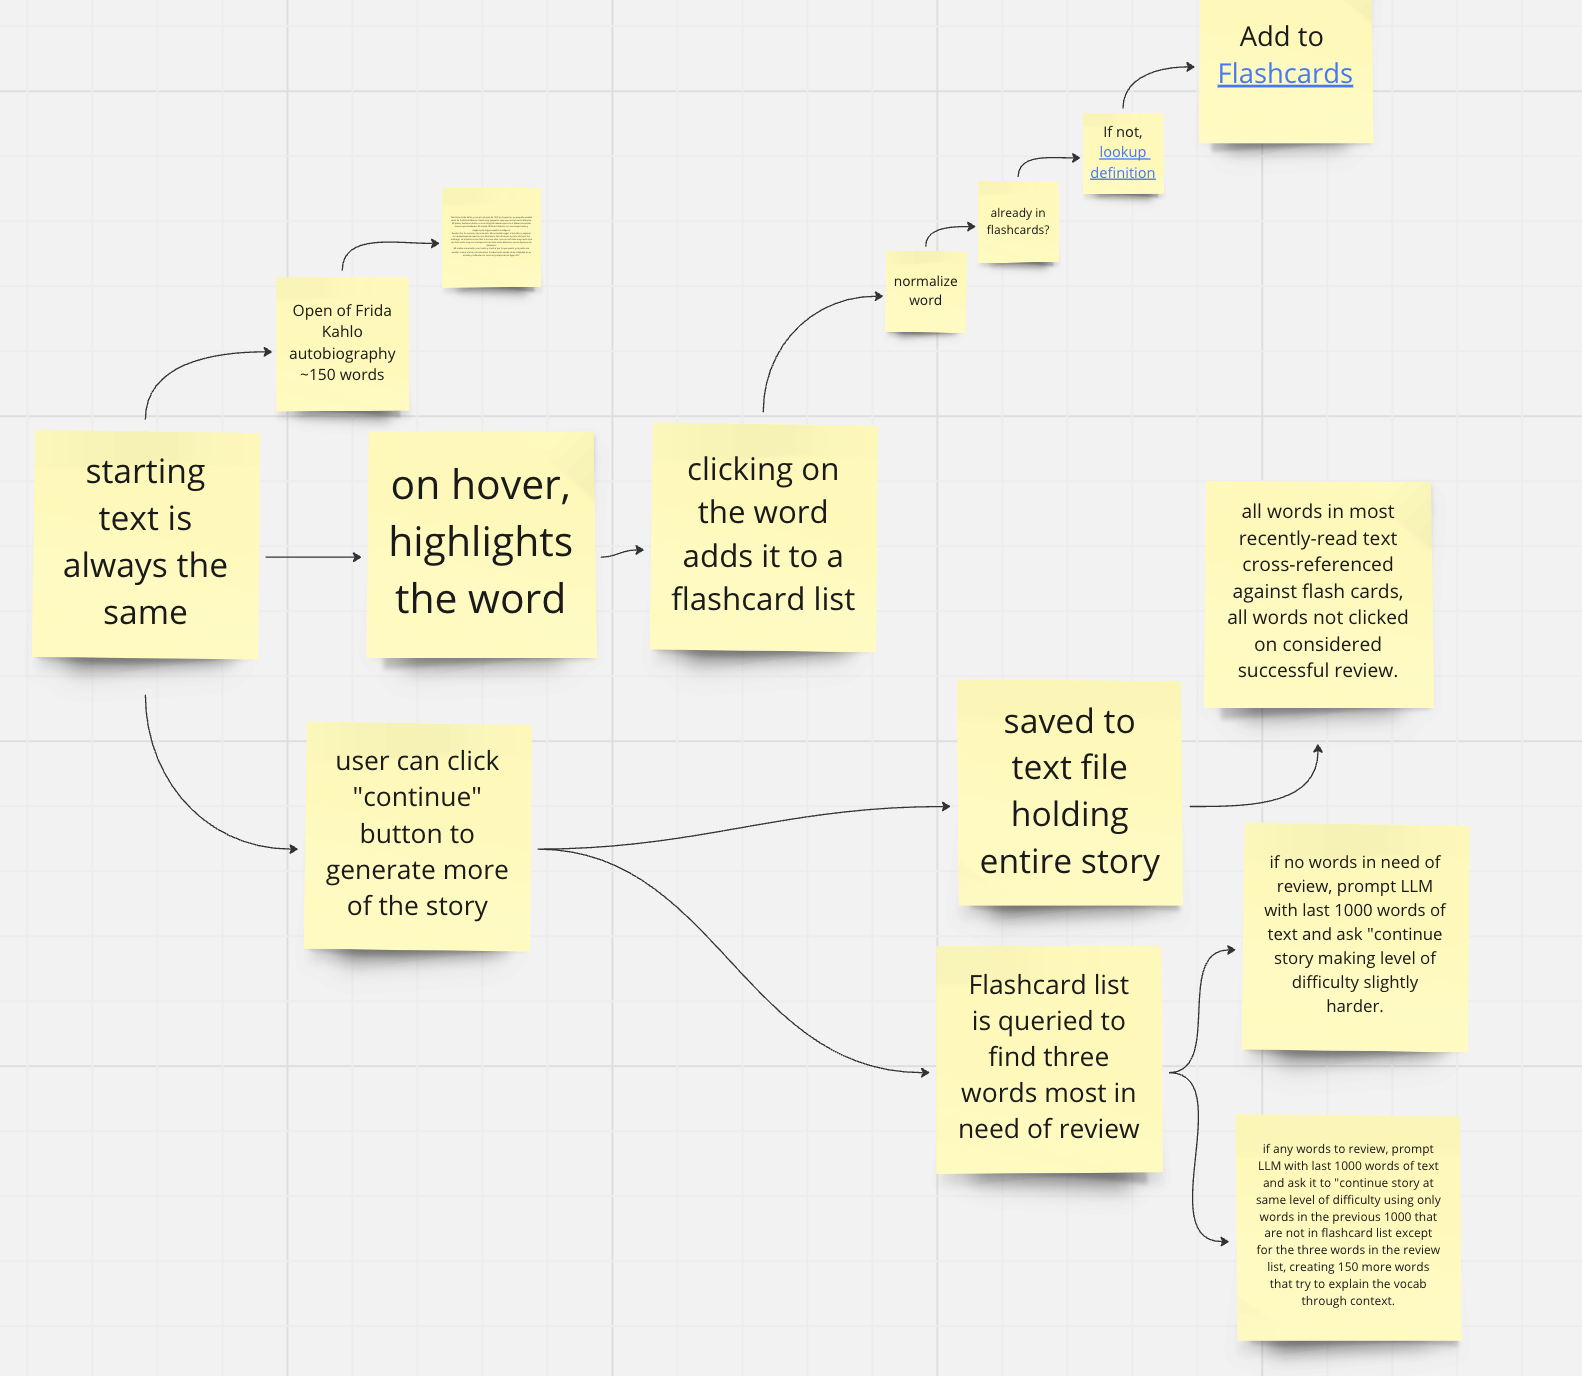
\includegraphics[width=0.5\linewidth]{Assignments//Assignment 2/design_sketch.png}
    \caption{Lazy Initial Project Diagram}
    \label{fig:enter-label}
\end{figure}

\section{Planning}
%In about half a page, provide a plan for what you expect to do next week. What threads or ideas will you pursue? What questions will you seek answers to in the literature?
I may struggle with my research log next week. I feel fairly confident about the direction and principles of my project and would actually prefer to spend a week building it to see which questions arise during the process. The obvious questions like what type of dictionary to use, which language to start with, how to blend spaced repetition into extensive reading, etc. feel at least generically answered. 

With this in mind, I may turn next week's attention to technical implementation details. Looking into the potential APIs for translations and flash cards was quite illuminating, although it will be increasingly difficult to glean that information from a diet of mostly research papers.

\printbibliography{}

\end{document}

